\documentclass[11pt]{article}
\usepackage{graphicx}
\usepackage[margin=12mm]{geometry}
\usepackage{sectsty}
\usepackage{subfigure}
\sectionfont{\fontsize{12}{10}\selectfont}

\begin{document}
\title{ECSE 526-Artificial Intelligence}
\author{Alexandre Coulombe}
\date{January 28, 2020}
\maketitle



\section{Total number of states explored}
The amount of nodes visited changes depending on the depth of the search. The three game states used for the evalution of the number of states explored using different depth configurations are described in figure \ref{fig:F0}.
 
\begin{figure}[h]
\centering
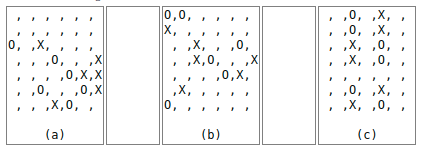
\includegraphics[scale=0.5]{Figure_0.png}
\caption{Game states used for the evalution of the number of states explored using different depth configurations}
\label{fig:F0}
\end{figure}

As expected, the number of states visited by the minimax algorithm is much greater than that of the alpha beta pruning algoritm. This is due to alpha beta pruning being an improvement on minimax using the idea of pruning to not explore states that do not impact the decision on the final move selected. This is because, when the player has found a better alternate move prior, a state will never be reached. So when enough information about a state is found to determined it will not be reached, it can be pruned. The data collected about the number of states explored by the program using various depths and the algorithms minimax and alpha beta pruning can be found in figure \ref{fig:F1}, \ref{fig:F2}, \ref{fig:F3}, \ref{fig:F4}, \ref{fig:F5} and \ref{fig:F6}.

%Add figure to document
\begin{figure}[ht]
\centering
\subfigure[Minimax]{\label{fig:F1}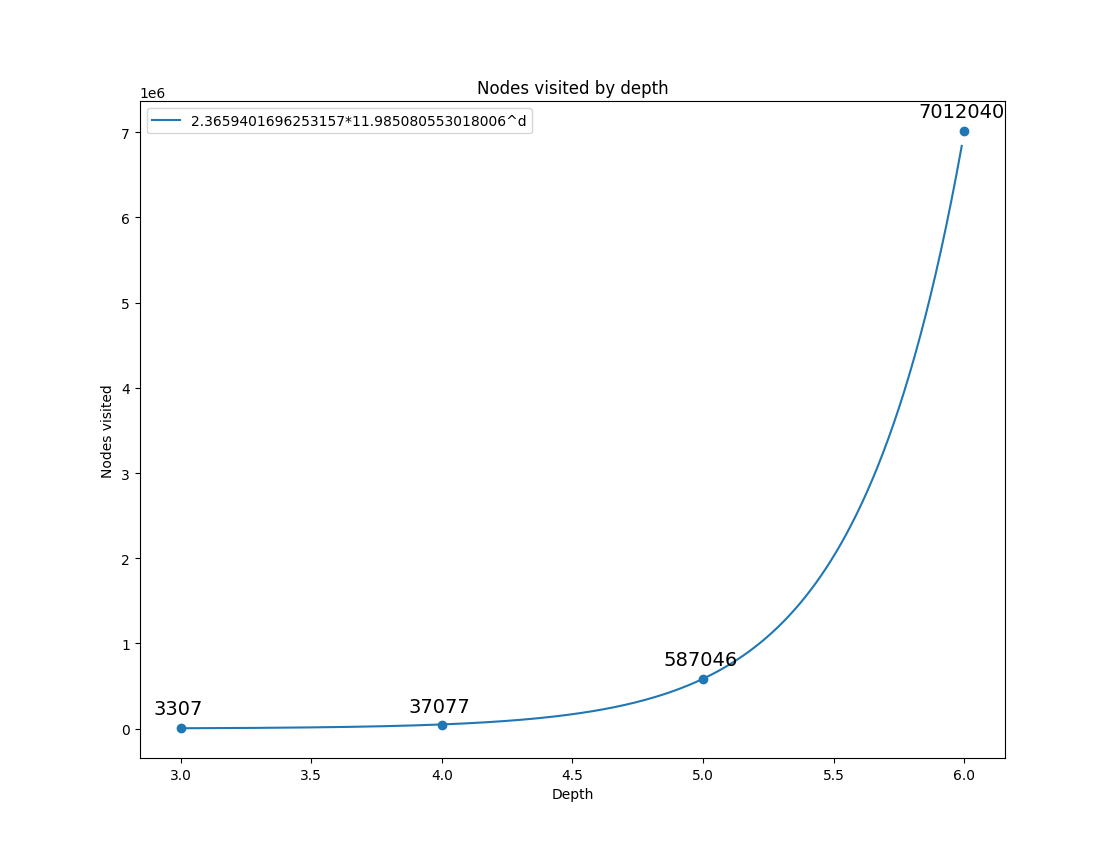
\includegraphics[width=0.35\textwidth, height=5cm]{Figure_1.png}}	
\subfigure[Alpha Beta Pruning]{\label{fig:F2}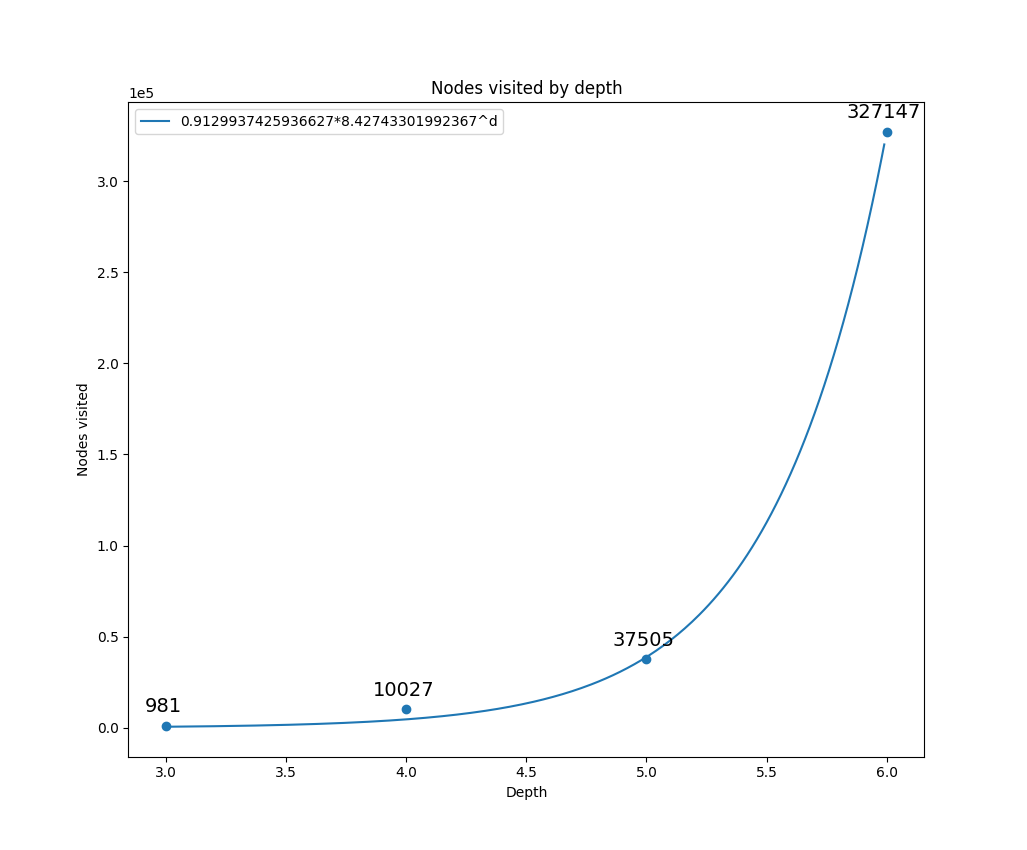
\includegraphics[width=0.35\textwidth, height=5cm]{Figure_2.png}}	
\caption{Nodes visited by depth of environment A using Minimax and Alpha Beta Pruning}
\end{figure}

%Add figure to document
\begin{figure}[ht]
\centering
\subfigure[Minimax]{\label{fig:F3}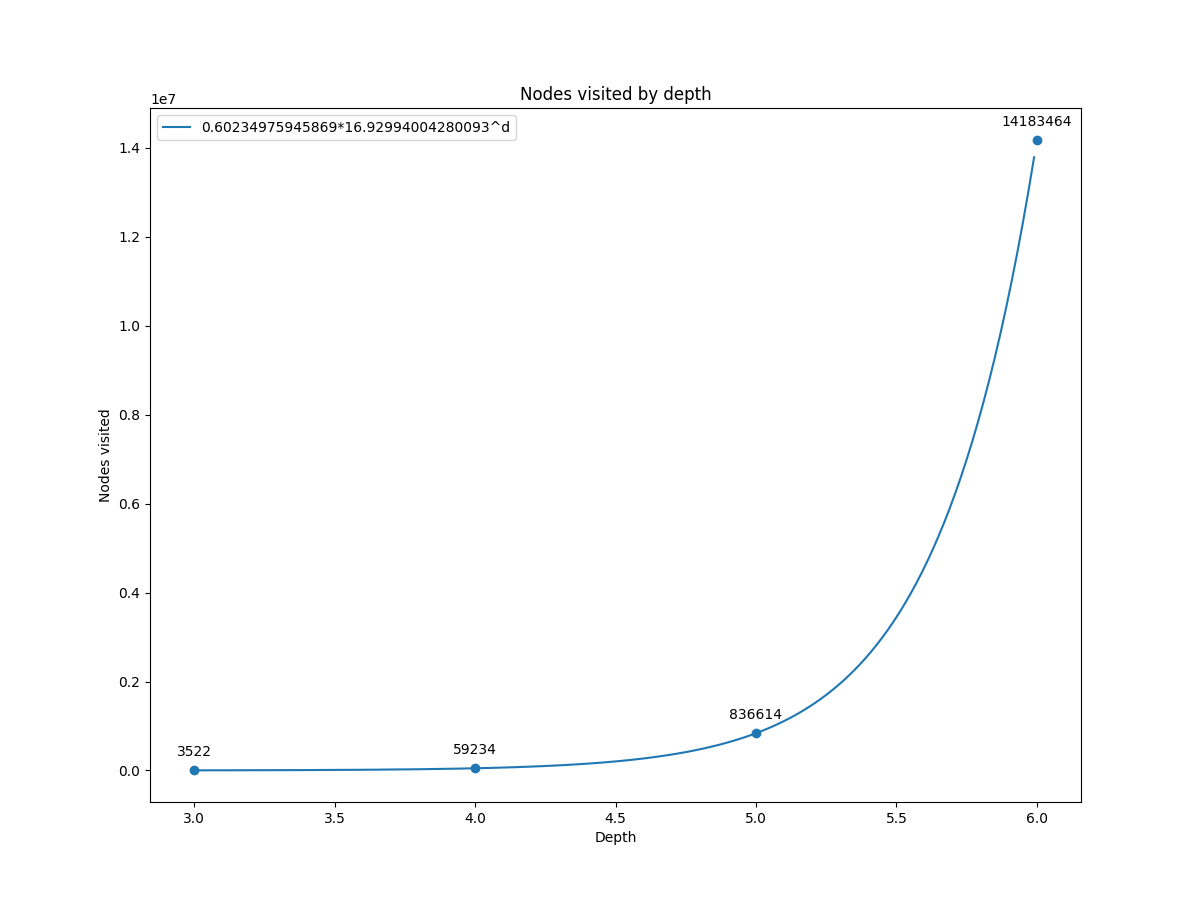
\includegraphics[width=0.35\textwidth, height=5cm]{Figure_3.png}}	
\subfigure[Alpha Beta Pruning]{\label{fig:F4}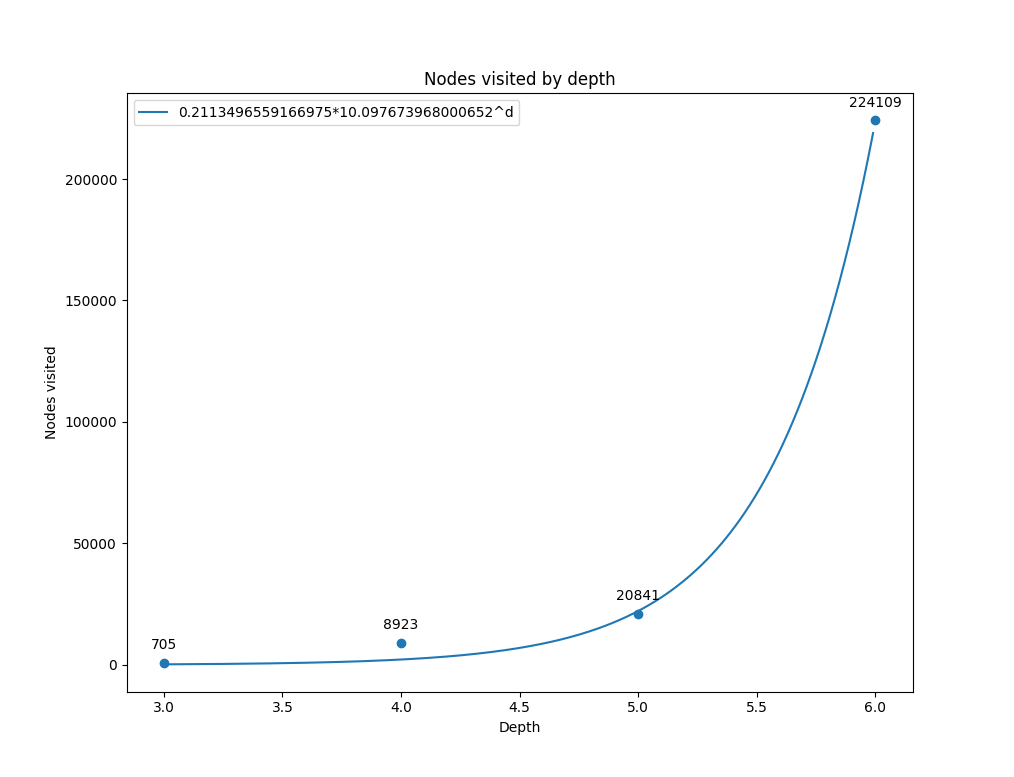
\includegraphics[width=0.35\textwidth, height=5cm]{Figure_4.png}}	
\caption{Nodes visited by depth of environment A using Minimax and Alpha Beta Pruning}
\end{figure}

%Add figure to document
\begin{figure}[ht]
\centering
\subfigure[Minimax]{\label{fig:F5}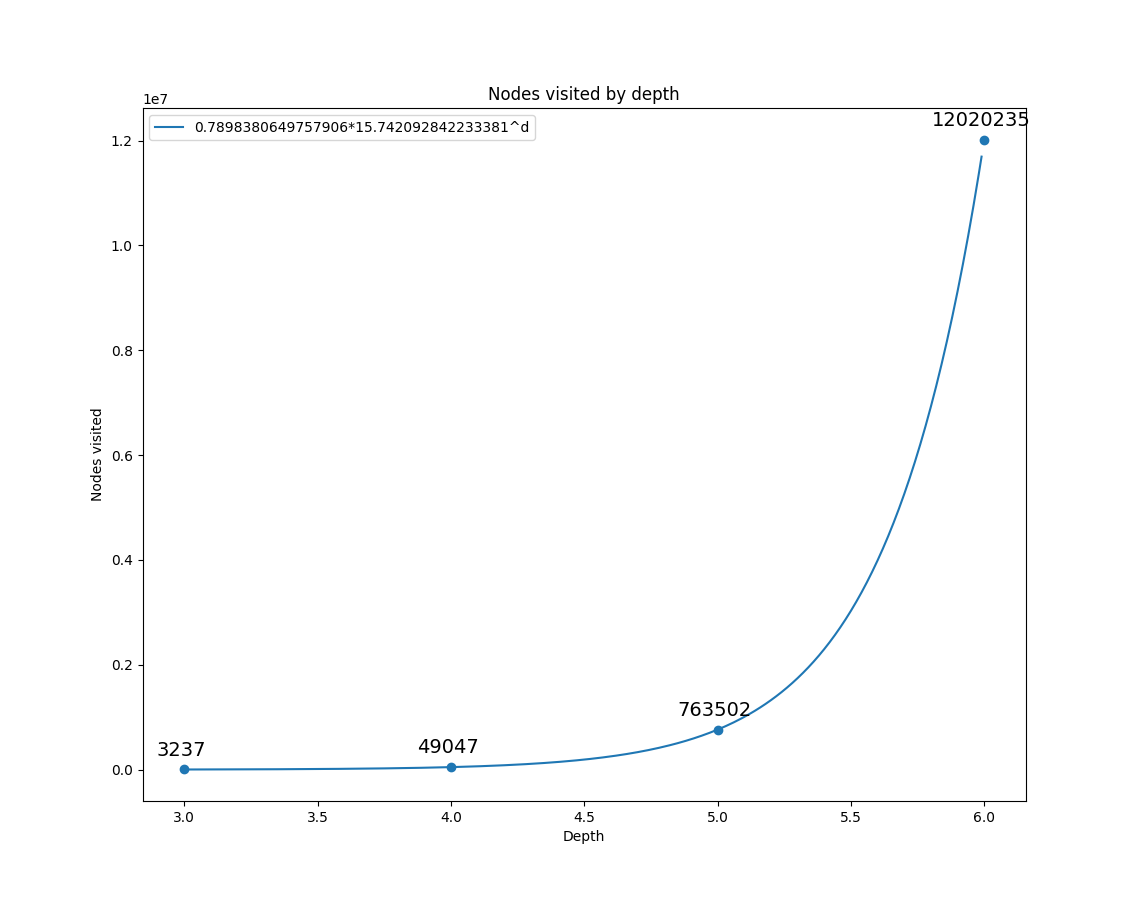
\includegraphics[width=0.35\textwidth, height=5cm]{Figure_5.png}}	
\subfigure[Alpha Beta Pruning]{\label{fig:F6}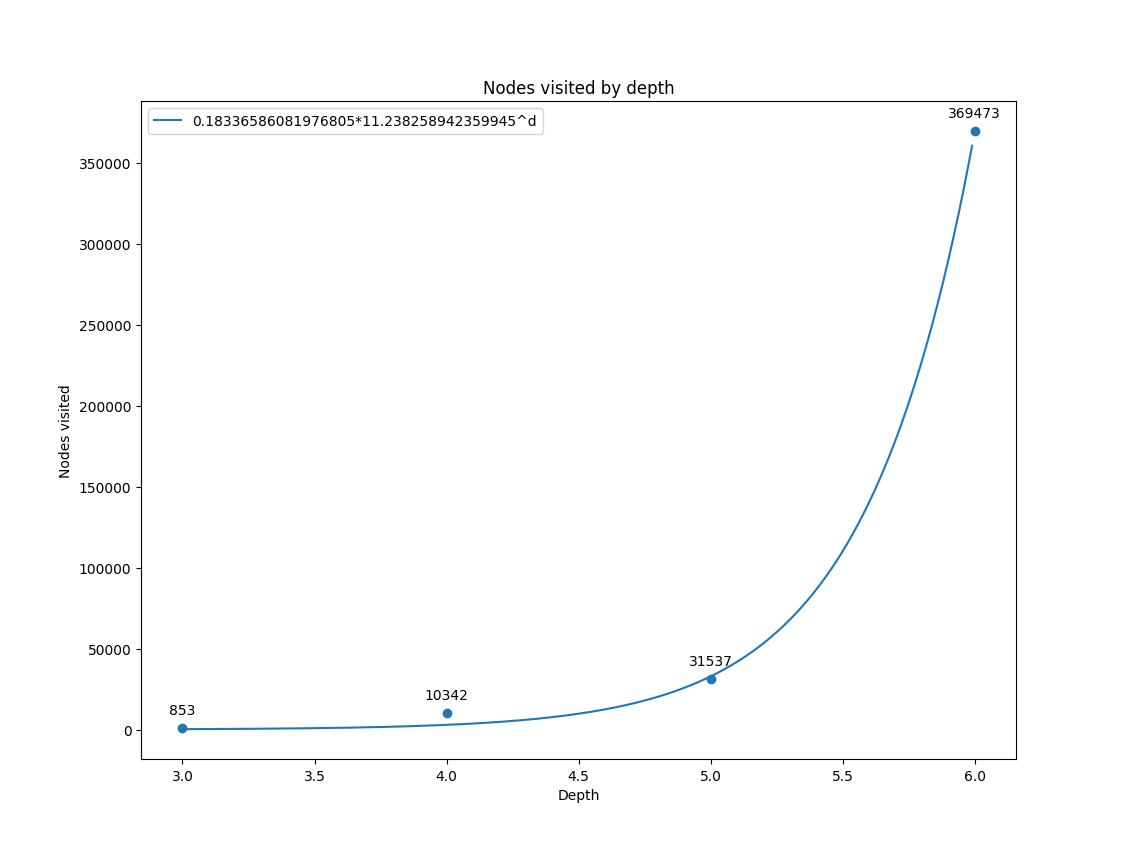
\includegraphics[width=0.35\textwidth, height=5cm]{Figure_6.png}}	
\caption{Nodes visited by depth of environment A using Minimax and Alpha Beta Pruning}
\end{figure}


\section{Depth cutoff to the number of states visited formula}

Due to the exponential nature of the data points, the formula $ states = a*b^d $ is used to estimate the relationship between the depth of the search and the number of nodes/states visited by the program. A curve fit was performed on each data set to find the values of the function that has the least squares error to the  values of the depth and corresponding visited nodes. For the minimax algorithm, the value for $a$ should be 1 in theory because there is only one starting state. The values found for the branching factor, $b$, are 11.985 for game state A, 16.923 for game state B and 15.742 for game state C. This gives an average of 14.883, which means, on average, each state has 14.883 possible moves. This would give the formula $ states = 14.883^d $ for the number of states visited for a certain depth $d$ by the minimax algorithm.

The alpha beta pruning data also shows an exponential form to it, so the estimated formula will also use the estimate $ states = a*b^d $. A curve fit was performed on each data set to find the values of the function that has the least squares error to the  values of the depth and corresponding visited nodes, as it was for minimax. For the alpha beta pruning algorithm, the value for $a$ should be 1 in theory because there is only one starting state. The values found for the branching factor, $b$, are 8.4274 for game state A, 10.0977 for game state B and 11.238 for game state C. This gives an average of 9.921, which means, on average, each state has $14.883-9.921=4.962$ possible moves and pruned. This would give the formula $ states = 9.921^d $ for the number of states visited for a certain depth $d$ by the minimax algorithm. 

\section{Generation order of new states}


\section{Heuristic evaluation function}
The heuristc evaluation function used by the program is a combination of two heuristics. The first heuristic is utility for the amount of pieces aligned, since the goal to win the game is to align four of your own pieces before your opponent does. The heuristic gives value based on the amount of pieces aligned. The value of two pieces being aligned is 1 point, the value of three pieces being aligned is 3 points and the value of four pieces being aligned is 1000, so that the agent will do the sequence to get the win. This heuristic gives utility to the program when it aligns pieces and a higher utility when it aligns even more pieces. This heuristic is to push the program to reach the goal of the game so that it is able to win against its opponent. If it were not included, the program would have any incentive to align pieces, which is the entire point of the game of dynamic connect 4.

The other heuristic used is the environment central dominance heuristic. The heuristic gives higher and higher value to pieces to get closer and closer to the center of the 
environment, in this case the center of the dynamic connect 4 game board. This gives the program incentive to move its pieces to the center of the board, and closer to each other in consequence. Due to the pieces being seperated at the start of the game on opposite sides of the game board, three on the left and three on the right, in order to align four pieces, at least one piece must traverse the board to reach the other pieces to align four pieces. However, by controlling the center of the board, more of your own pieces will be closer to each other, which allows the program to find states which align the pieces. The values of the tiles are saved in a 2D array assigning higher and higher value to tiles getting closer and closer to the center, with the center having the highest value.

By combining both of the heuristics together, the program will choose actions that have the highest utility, which means moves that move pieces to the center of the board and align pieces that are near each other will be played. However, if we consider the utility of the opponent's moves, we can find states in which we have a higher utility and the opponent has lower utility and perform the sequence of actions to reach those states. This makes the final heuristic $ player heuristic - opponent heuristic $, which allows the player to play moves that benefit it and disadvantage the opponent. 
\section{Simple vs Complex evaluation function}

\end{document}